\subsection{Teorema Pythagoras}
Salah satu teorema paling terkenal di kalangan awam (atau setidaknya di pop culture). Diberikan segitiga $ABC$ dengan sudut $C$ siku-siku. Jika panjang sisi $AB=c$, $BC=a$, dan $CA=b$, maka berlaku
\begin{align*}
    a^2+b^2=c^2
\end{align*}
\begin{center}
    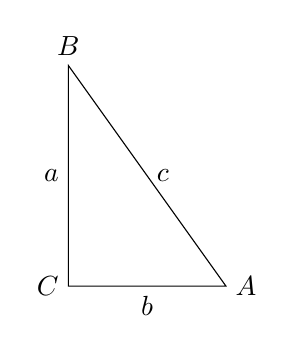
\begin{tikzpicture}
    % titik-titik segitiga
    \coordinate[label=left:$C$]  (C) at (-1.5cm,-1.cm);
    \coordinate[label=above:$B$] (B) at (-1.5cm,1.8cm);
    \coordinate[label=right:$A$] (A) at (0.5cm,-1.cm);
    
    % pembuatan segitiga
    \draw (A) -- node[right]{$c$} (B)  -- node[left]{$a$} (C) -- node[below]{$b$} cycle;
    \end{tikzpicture}
\end{center}